\documentclass[11pt,a4paper]{article}

\usepackage[utf8]{inputenc}
\usepackage[T1]{fontenc}
\usepackage[english]{babel}
\usepackage[a4paper,margin=2.4cm]{geometry}

\usepackage{amsmath, amssymb, amsthm}
\usepackage{mathtools}
\usepackage{stmaryrd}
\usepackage{booktabs}
\usepackage{tabularx}
\usepackage{array}
\usepackage{caption}
\usepackage{subcaption}
\usepackage{float}
\usepackage{enumitem}
\usepackage{microtype}
\usepackage{xcolor}
\usepackage{listings}
\usepackage{fancyhdr}
\usepackage{titlesec}
\usepackage{graphicx}
\usepackage{tikz}
\usetikzlibrary{positioning, arrows.meta, fit, backgrounds, calc, shapes.geometric}
\usepackage[hidelinks]{hyperref}

%  ---  Palette shared with the companion reports  ---
\definecolor{ink}{RGB}{26,30,36}
\definecolor{slate}{RGB}{92,101,112}
\definecolor{mist}{RGB}{233,235,238}
\definecolor{rulegrey}{RGB}{188,194,201}
\definecolor{steel}{RGB}{47,72,102}
\definecolor{steellight}{RGB}{124,146,172}
\definecolor{signal}{RGB}{160,32,45}
\definecolor{southc}{RGB}{51,115,204}
\definecolor{northc}{RGB}{230,128,38}
\definecolor{knows}{RGB}{26,140,70}

\hypersetup{
    colorlinks=true,
    linkcolor=steel,
    citecolor=steel,
    urlcolor=steel,
    pdftitle={Where to Look From},
    pdfauthor={Haniel Ulises},
}

\color{ink}

\setlength{\headheight}{22pt}
\pagestyle{fancy}
\fancyhf{}
\fancyhead[L]{\small\textcolor{slate}{\itshape Where to Look From}}
\fancyhead[R]{\small\textcolor{slate}{\thepage}}
\renewcommand{\headrulewidth}{0.4pt}
\renewcommand{\headrule}{\hbox to\headwidth{\color{rulegrey}\leaders\hrule height \headrulewidth\hfill}}

\titleformat{\section}{\normalfont\large\bfseries\color{ink}}{\thesection}{0.7em}{}
\titleformat{\subsection}{\normalfont\normalsize\bfseries\color{ink}}{\thesubsection}{0.7em}{}
\titleformat{\paragraph}[runin]{\normalfont\bfseries\color{slate}}{}{0em}{}[.]

\captionsetup{font=small, labelfont={bf,color=slate}, textfont=footnotesize}

\theoremstyle{definition}
\newtheorem{definition}{Definition}
\newtheorem{proposition}{Proposition}
\newtheorem{lemma}{Lemma}
\newtheorem{corollary}{Corollary}
\newtheorem{fact}{Fact}
\newtheorem{remark}{Remark}

\lstdefinestyle{sys}{
    backgroundcolor=\color{mist},
    basicstyle=\ttfamily\scriptsize\color{ink},
    keywordstyle=\color{steel}\bfseries,
    commentstyle=\color{slate}\itshape,
    stringstyle=\color{slate},
    morecomment=[l]{;},
    morekeywords={:types,:predicates,:objects,:agents,:goal,:init,:event,:action,:action-type,:observability-conditions,:precondition,:effects,:events,:relations,:designated,:conditions,:observability-types},
    frame=single,
    rulecolor=\color{rulegrey},
    framesep=5pt,
    xleftmargin=6pt,
    xrightmargin=0pt,
    breaklines=true,
    showstringspaces=false,
    columns=fullflexible,
    captionpos=b,
}
\lstset{style=sys}

%  ---  Notation  ---
\newcommand{\Ag}{\mathcal{A}}
\newcommand{\Mod}{\mathcal{M}}
\newcommand{\Ev}{\mathcal{E}}
\newcommand{\prd}{\otimes}
\newcommand{\Kop}[1]{K_{#1}}
\newcommand{\Eop}[1]{E_{#1}}
\newcommand{\Cop}[1]{C_{#1}}
\newcommand{\Kw}[1]{\mathit{Kw}_{#1}}
\newcommand{\code}[1]{\texttt{\small #1}}
\newcommand{\ag}[1]{\mathit{#1}}
\newcommand{\job}{\mathit{job}}
\newcommand{\pre}{\mathit{pre}}
\newcommand{\post}{\mathit{post}}
\newcommand{\dist}{\mathrm{dist}}
\newcommand{\depth}{\mathrm{depth}}

\newcommand{\tap}[1]{\mathit{tapado\text{-}#1}}
\newcommand{\bz}{\mathit{blocked\text{-}z}}
\newcommand{\atm}[1]{\mathit{at\text{-}m}_{#1}}
\newcommand{\act}[1]{\textsf{#1}}

\begin{document}

\begin{titlepage}
\centering
\vspace*{2.4cm}
{\color{rulegrey}\rule{\textwidth}{0.8pt}}\\[0.9cm]
{\LARGE\bfseries Where to Look From\par}
\vspace{0.5cm}
{\large\color{slate} Knowing Whether, a Sensing Action with a Modal Precondition,\\
and Two Lookouts, One of Them Perhaps Screened\par}
\vspace{0.7cm}
{\color{rulegrey}\rule{\textwidth}{0.8pt}}\\[1.4cm]

{\large Haniel Ulises\par}
\vspace{0.3cm}
{\color{slate} Epistemic Robotics}\\
\vspace{0.15cm}
{\color{slate}13 October 2026}

\vfill
{\color{slate}\small
A robot must know whether a zone is blocked. It can see the zone from either of
two lookouts, and a screen may stand in front of one of them, never both; the
robot does not know which. A look through a screen decides nothing, and a look
from lookout $k$ is written with the precondition that the robot know the view
from $k$ is clear. We prove that this domain has no conformant plan: no sequence
of its actions is applicable in every world and reaches the goal, because the
precondition of every look is false in two of the six worlds. A policy of five
nodes reaches the goal in all six, and drives to the second lookout in exactly
the two worlds with a screen at the first. In the world, any sequence either
drives to the second lookout in every run or leaves the zone unobserved behind a
screen. Thirty paired seeds per formulation in Gazebo measure this: the policy's success is backed by the map the
robot built in 30 of 30 runs, and it drives to the second lookout in 10; the
classical sequence committed to the first lookout reports success in 30 and is
backed in 20, every unbacked run behind a screen with no cell of the zone
observed (McNemar's exact $p = 0.002$); the sequence through both lookouts is
backed in 30 and slower in every pair, by a Hodges--Lehmann estimate of
26.6\,s.}
\vspace{1.2cm}
\end{titlepage}

\tableofcontents
\newpage

%  ======================================================================
\section{Scope}

This report states one scenario of a harness for repeated simulator runs, and
the film recorded of it for the Epistemic Robotics site. The scenario, its
launch file, the harness that runs and measures it and the batch of runs are
not in this repository; the domain is restated here in notation, and every
figure is computed from the batch's table of runs. The film's four takes were
recorded with the harness unchanged.

The question the scenario asks is narrow. A look that can end without deciding
is a problem when noise is its cause: an outcome that may occur in any world
leaves no policy that guarantees the goal.
Here the undecided look has a cause the robot can observe, a screen across the
sight line, and the planner can choose where to look from. The planning is
epistemic planning over dynamic epistemic logic~\cite{ba2011}, with a goal of
knowing whether~\cite{fhmv1995,pb2002}.

%  ======================================================================
\section{The domain}

One agent, $r1$. Five atoms: $\bz$, the zone is blocked; $\tap{1}$ and
$\tap{2}$, a screen hides the zone from lookout 1 or 2; $\atm{1}$ and
$\atm{2}$, the robot is at lookout 1 or 2. Five actions, each an event model in
the sense of Baltag, Moss and Solecki~\cite{bms1998}:

\begin{center}
\small
\begin{tabularx}{\textwidth}{@{}l l X X@{}}
\toprule
action & kind & precondition & events \\
\midrule
\act{goto-m1}, \act{goto-m2} & public ontic & $\neg\atm{k}$ & $\atm{k}$ becomes true and the other false \\
\act{vista-1} & sensing & $\atm{1}$ & \act{e-vista1-tapada} where $\tap{1}$, \act{e-vista1-despejada} where $\neg\tap{1}$ \\
\act{mirar-1} & sensing & $\atm{1} \wedge K_{r1}\neg\tap{1}$ & \act{e-mirar1-bloqueada} where $\bz$, \act{e-mirar1-libre} where $\neg\bz$ \\
\act{mirar-2} & sensing & $\atm{2} \wedge K_{r1}\neg\tap{2}$ & the same, from lookout 2 \\
\bottomrule
\end{tabularx}
\end{center}

\noindent
The sensing actions are semi-private: $r1$ distinguishes the events, and any
other agent would see only that the action took place. The initial model is the
six valuations of $(\bz, \tap{1}, \tap{2})$ with $\neg(\tap{1} \wedge \tap{2})$
and $\neg\atm{1} \wedge \neg\atm{2}$, all six designated, and $r1$'s relation the
universal one; the frame is S5. The goal is $\Kw{r1}\,\bz$, that is,
$K_{r1}\bz \vee K_{r1}\neg\bz$. That at most one view is screened, being true in
every world of an S5 model in which $r1$ relates all worlds, is common
knowledge.

There is no action that checks the view from lookout 2. The two propositions
below show why none is needed.

%  ======================================================================
\section{The hall}

\begin{figure}[H]
\centering
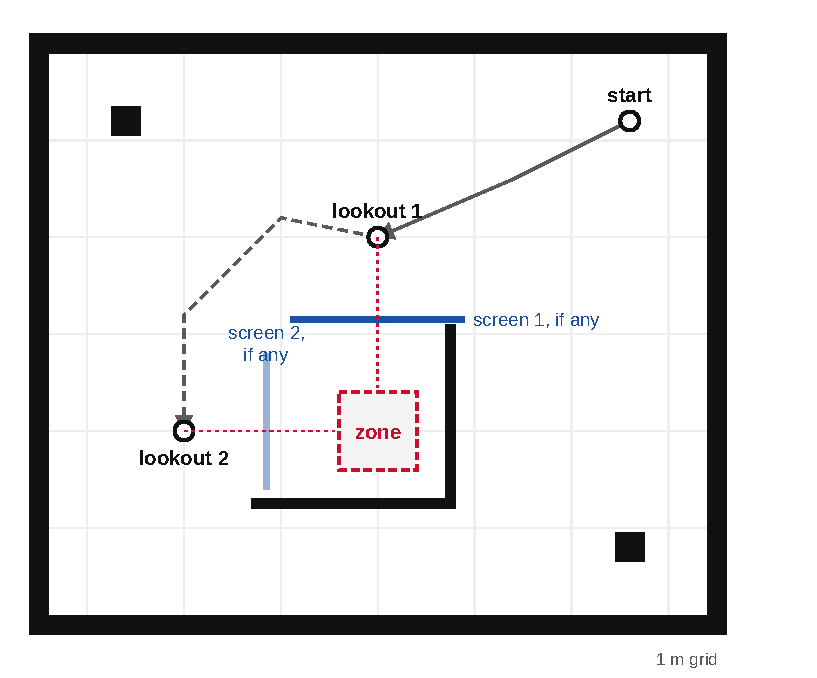
\includegraphics[width=0.5\textwidth]{figures/two_lookouts_floor.pdf}
\caption{The hall, 7 by 6\,m. The zone is a 0.8\,m square at the origin with
back walls to its south and east; lookout 1 stands 2\,m north of it and
lookout 2 stands 2\,m west. The two bars mark where a screen may stand, at
$y = 1.15$\,m and $x = -1.15$\,m; at most one holds one. The solid route goes
from the start to lookout 1, and the dashed one, from lookout 1 to lookout 2,
is driven only behind a screen.}
\label{fig:hall}
\end{figure}

\noindent
The back walls are not decoration: a laser certifies a cell free only along a
ray that ends on something, and the rays that cross the zone end on them. In the
blocked worlds a 0.35\,m crate stands in the zone. The robot is a TurtleBot3
Burger mapping the hall with slam\_toolbox from a start in the north-east corner,
perturbed by the seed by up to 0.2\,m on each axis and $10^\circ$ in heading.
Six worlds rotate over the seeds, seed $s$ taking world $s \bmod 6$, so thirty
seeds give each world five runs.

%  ======================================================================
\section{No conformant plan, and a policy}

\begin{proposition}[No conformant plan]
\label{prop:noconf}
No sequence of the domain's actions is applicable in all six initial worlds and
leaves $\Kw{r1}\,\bz$ true in all of them.
\end{proposition}

\begin{proof}
Initially $\Kw{r1}\,\bz$ is false, since $r1$ relates a world where $\bz$ holds
to one where it does not. The only actions whose events differ on $\bz$ are
\act{mirar-1} and \act{mirar-2}; every other action leaves $r1$'s relation
between two worlds that differ on $\bz$ in place, so a sequence that reaches the
goal contains a look. Consider the first look in it, \act{mirar-$k$}. For the
sequence to be applicable in every world, its precondition must hold in the
state reached from every world, and in particular from a world where $\tap{k}$
holds. No action changes $\tap{k}$, so $\tap{k}$ still holds there, and since
the frame is S5, $K_{r1}\neg\tap{k}$ implies $\neg\tap{k}$: the precondition is
false. Such a world exists for $k = 1$ and for $k = 2$.
\end{proof}

\begin{proposition}[The policy]
\label{prop:policy}
The policy
\[
\act{goto-m1};\ \act{vista-1};\
\begin{cases}
\act{e-vista1-tapada}: & \act{goto-m2};\ \act{mirar-2}\\
\act{e-vista1-despejada}: & \act{mirar-1}
\end{cases}
\]
is applicable in all six worlds, reaches $\Kw{r1}\,\bz$ in all six, and executes
\act{goto-m2} in exactly the two worlds where $\tap{1}$ holds.
\end{proposition}

\begin{proof}
\act{goto-m1} and \act{vista-1} are applicable everywhere. If $\tap{1}$ holds,
\act{e-vista1-tapada} occurs and the designated worlds become the two where
$\tap{1}$ holds; in both, $\neg\tap{2}$, so $K_{r1}\neg\tap{2}$ holds after
\act{goto-m2}, which changes no screen, and \act{mirar-2} is applicable. If
$\neg\tap{1}$, \act{e-vista1-despejada} occurs, the designated worlds are the
four where $\neg\tap{1}$, and \act{mirar-1} is applicable. In either branch the
look's two events split the designated worlds by $\bz$, and whichever occurs,
$r1$ relates only worlds that agree on it. \act{goto-m2} lies only on the first
branch.
\end{proof}

\noindent
The precondition $K_{r1}\neg\tap{k}$ is what makes the difference between the
two propositions: it is the weakest condition under which a look from $k$ is
certain to decide the zone, and it is unknown until the robot has looked. The
branch on \act{vista-1} is where the robot finds out, and the elimination in the
first branch, from $\tap{1}$ and $\Cop{}\neg(\tap{1} \wedge \tap{2})$ to
$K_{r1}\neg\tap{2}$, is why no check of lookout 2 is needed.

\paragraph{Classical plans}
A classical planner given the task without knowledge has looks with no modal
precondition: \code{look\_into} requires only that the robot stand at a lookout,
and lasts its declared 8\,s. The two plans compared are POPF's for
the goal of having looked from lookout 1, a sequence of two actions, and for the
goal of having looked from both, a sequence of four. In the world, a look from
lookout $k$ behind a screen observes no cell of the zone. So, as in the proof of
Proposition~\ref{prop:noconf}, a sequence that leaves the zone observed in every
world contains a look from lookout 2 and drives there in every world, and one
that does not drive there leaves the zone unobserved in the two worlds with a
screen at lookout 1.

%  ======================================================================
\section{On the robot}

The harness launches the PlanSys2 stack with ePlanSys's epistemic state,
perception and executor, slam\_toolbox, and the action nodes of the six-room
demonstration, reused with other parameters; it adds a recorder of the map, the
actions and the true pose, and a mission node that sends the order and records
the outcome. The perception watches three regions of the occupancy grid: the
strip where screen 1 would stand, and the zone, once for each look. A region is
blocked when one of its cells is occupied, clear when every cell is free, and
undecided otherwise. Each region answers one sensing action, and the epistemic
state applies an observation only when its event is applicable.

The epistemic look action turns the robot to the region and returns when the
epistemic state reports $\Kw{r1}$ of the action's atom. On the recorded runs
that happened on the first grid after the robot faced the region, and the action
took between 0.2 and 2.3\,s. A run is \emph{backed} when the map the robot built
classifies the zone, by the same rule, as the robot reported.

%  ======================================================================
\section{Thirty seeds}

Each seed fixes the world, the start pose and the laser noise, 0.01\,m, and is
run under all three formulations, so the comparison is paired. Times are in
simulated seconds, from the order to the end of the mission.

\begin{table}[H]
\centering
\footnotesize
\begin{tabular}{@{}lccccc@{}}
\toprule
& reports success & backed by the map & to lookout 2 & median time & median path \\
\midrule
epistemic & 30/30 & \textbf{30/30} & \textbf{10/30} & \textbf{15.1\,s} & 2.71\,m \\
classical, one lookout & 30/30 & 20/30 & 0/30 & 22.8\,s & 2.63\,m \\
classical, both lookouts & 30/30 & 30/30 & 30/30 & 51.2\,s & 6.28\,m \\
\bottomrule
\end{tabular}
\caption{The batch, thirty seeds per formulation.}
\end{table}

\begin{table}[H]
\centering
\small
\begin{tabular}{@{}llccc@{}}
\toprule
world & epistemic looks & epistemic & classical, one & classical, both \\
\midrule
clear, screen 1 & \act{vista-1}, \act{mirar-2} & 5/5 $\cdot$ 34.9\,s & \textbf{0/5} $\cdot$ 22.5\,s & 5/5 $\cdot$ 51.2\,s \\
blocked, screen 1 & \act{vista-1}, \act{mirar-2} & 5/5 $\cdot$ 35.6\,s & \textbf{0/5} $\cdot$ 22.8\,s & 5/5 $\cdot$ 51.9\,s \\
clear, no screen & \act{vista-1}, \act{mirar-1} & 5/5 $\cdot$ 14.5\,s & 5/5 $\cdot$ 22.6\,s & 5/5 $\cdot$ 50.8\,s \\
blocked, no screen & \act{vista-1}, \act{mirar-1} & 5/5 $\cdot$ 14.4\,s & 5/5 $\cdot$ 22.4\,s & 5/5 $\cdot$ 50.7\,s \\
clear, screen 2 & \act{vista-1}, \act{mirar-1} & 5/5 $\cdot$ 15.1\,s & 5/5 $\cdot$ 23.0\,s & 5/5 $\cdot$ 51.4\,s \\
blocked, screen 2 & \act{vista-1}, \act{mirar-1} & 5/5 $\cdot$ 14.9\,s & 5/5 $\cdot$ 22.8\,s & 5/5 $\cdot$ 51.3\,s \\
\bottomrule
\end{tabular}
\caption{By world: runs backed by the map, and the median time.}
\end{table}

\noindent
The ten unbacked classical runs are the ten behind screen 1: the map holds the
screen's place as blocked and no cell of the zone as observed, and the mission
reports success. On backed success the discordant pairs are 10 to 0, and
McNemar's exact test~\cite{mcnemar1947} gives $p = 0.002$. Against the classical
plan through both lookouts every paired difference in time favours the policy,
with a Hodges--Lehmann estimate~\cite{hl1963} of 26.6\,s; against the one-lookout
plan the differences change sign with the world, the policy being faster in the
four worlds it decides from lookout 1, by about 8\,s, since its looks end on
knowledge, and slower by about 12\,s in the two it is forced to lookout 2. No
run of any formulation reported the zone with the wrong class, and every mission
ended in success.

%  ======================================================================
\section{The film}

Four takes, recorded one at a time on a ROS domain and Gazebo port of their own,
with the harness unchanged and headless: a Gazebo client and RViz on a virtual
display, the world held paused until both had drawn, and the Gazebo camera cut
on the executor's own actions.

\begin{table}[H]
\centering
\footnotesize
\setlength{\tabcolsep}{4pt}
\begin{tabular}{@{}lllccl@{}}
\toprule
take & world & looks & reports & sim time & the zone on the map \\
\midrule
epistemic, seed 1 & clear, screen 1 & \act{vista-1}, \act{mirar-2} & SUCCESS & 34.9\,s & 256 of 256 cells, clear \\
classical, one, seed 1 & clear, screen 1 & \act{mirar-1} & SUCCESS & 22.3\,s & 0 of 256 cells, unknown \\
classical, both, seed 1 & clear, screen 1 & \act{mirar-1}, \act{mirar-2} & SUCCESS & 51.1\,s & 256 of 256 cells, clear \\
epistemic, seed 3 & clear, no screen & \act{vista-1}, \act{mirar-1} & SUCCESS & 14.3\,s & 256 of 256 cells, clear \\
\bottomrule
\end{tabular}
\caption{The film's takes.}
\end{table}

\begin{figure}[H]
\centering
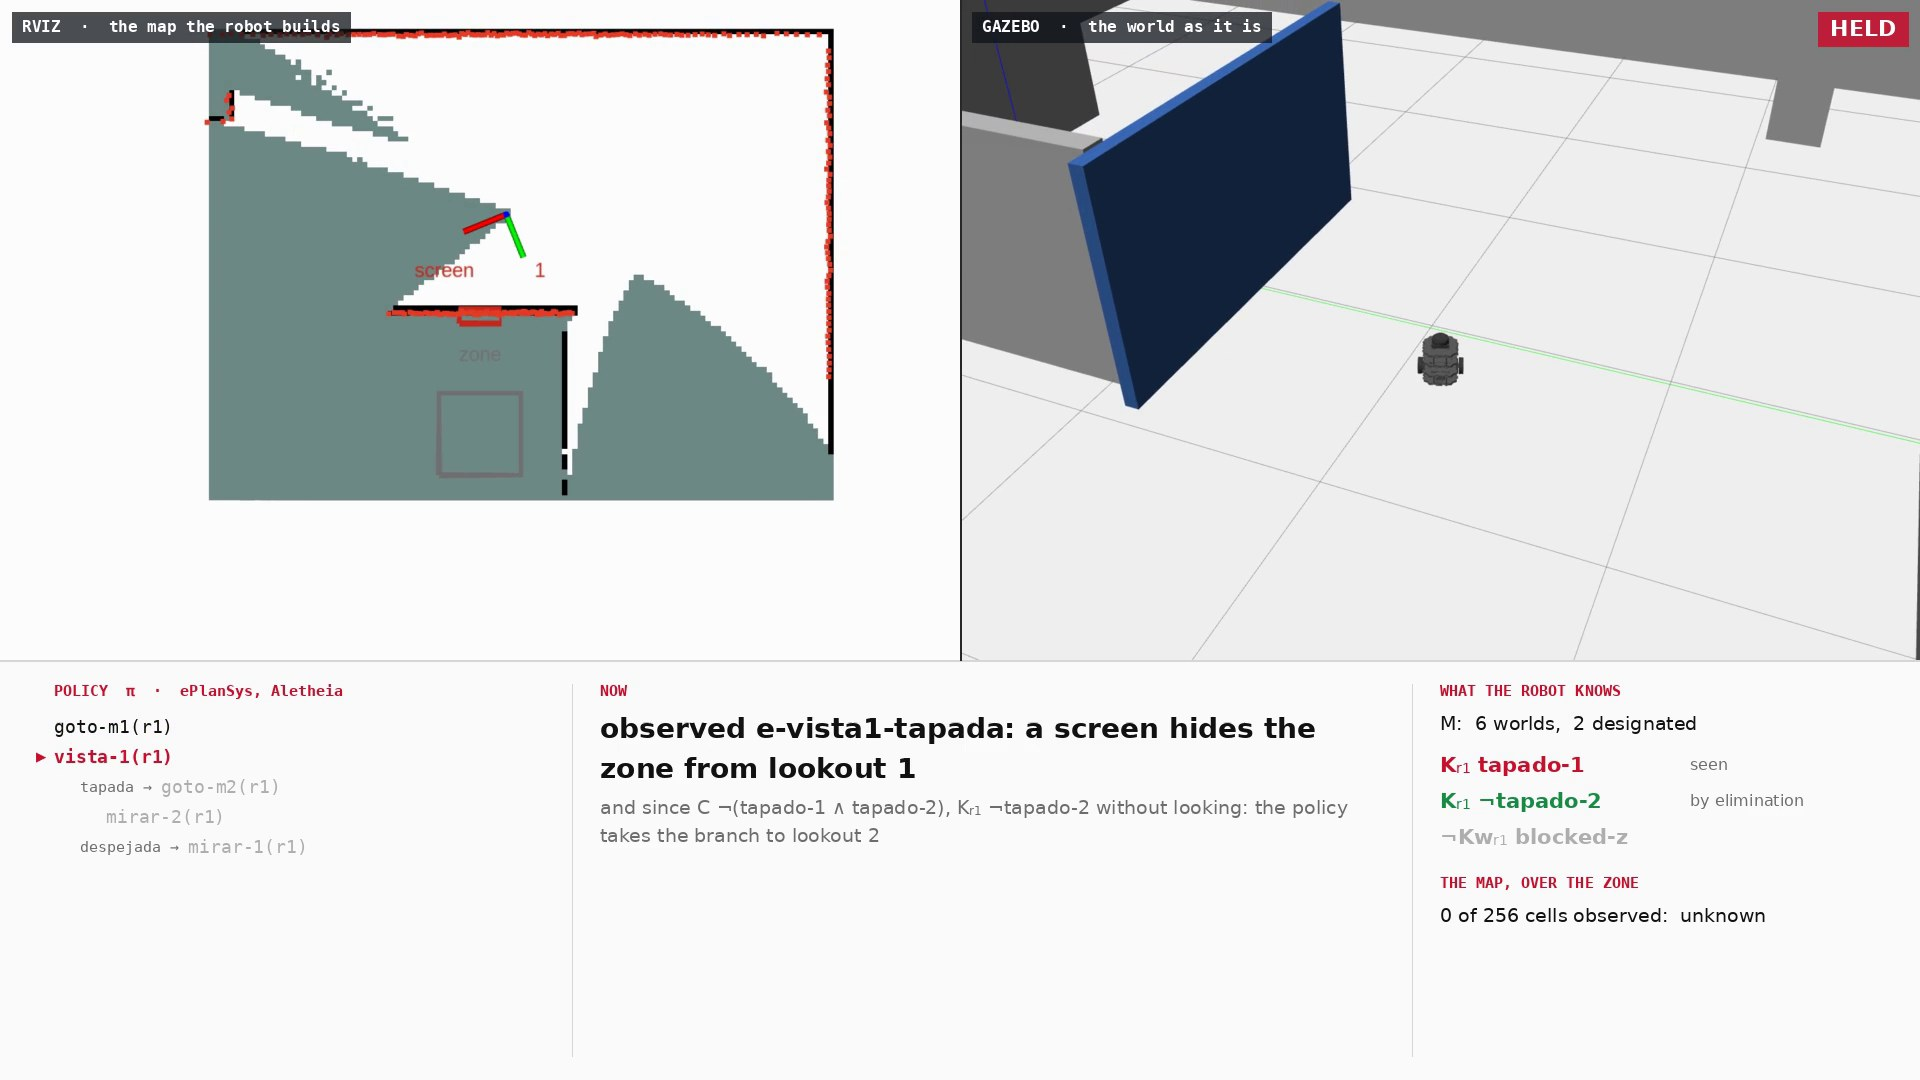
\includegraphics[width=\textwidth]{figures/two_lookouts_frame.jpg}
\caption{The film at the screen on seed 1, held. Left, RViz: the map, with the
screen's place outlined red, blocked, and the zone grey, undecided. Right,
Gazebo: the robot at lookout 1 before the screen. Under both: the policy with
\act{vista-1} running and its branches, the observation, and what the robot
knows: $K_{r1}\tap{1}$ seen, $K_{r1}\neg\tap{2}$ by elimination, and the zone
still unknown, with 0 of its 256 cells observed.}
\end{figure}

\noindent
Every figure on the film's panels is a line one of the runs wrote. The model's
counts on the recorded runs went from 6 designated worlds to 2 at the screen
and to 1 at the zone on seed 1, and from 6 to 4 and to 2 on seed 3, where
whether a screen stands at lookout 2 remains open and no longer matters.

\paragraph{Two timings found on the way}
The executor reports an observed outcome after the epistemic state has applied
it; on seed 3 after the zone's observation too, since there the zone was in view
from lookout 1, and the state applied \act{e-mirar1-libre} at the same instant
as \act{e-vista1-despejada}, as soon as $K_{r1}\neg\tap{1}$ made it applicable.
\act{mirar-1} then ran and returned in 0.2\,s. A first cut of the film timed its
captions from the executor's reports and so showed the model a step ahead at the
clear view; the published film times them from the epistemic state. The log of
every epistemic run also repeats that \act{mirar-1\_r1} is not applicable: it is
the zone's region for the look not in progress, offered and refused, and it
changes nothing.

%  ======================================================================
\section{What this does not show}

\begin{itemize}[leftmargin=1.4em]
\item A stronger classical agent. A classical planner inside a loop that
monitors execution and replans when a look does not decide would also reach the
zone behind a screen. It would need the condition the epistemic domain writes as
a precondition written into the monitor, and what a look decides written into
the replanning.
\item Noise that confuses a screen with a clear view. At 0.01\,m the regions
decided correctly in every run; noisier lasers were not run here.
\item More than one robot, or more than two lookouts. Neither was built or
measured.
\item Localisation. The map is built with the simulator's odometry, and the
world frame is the map frame.
\end{itemize}

%  ======================================================================
\begin{thebibliography}{9}
\bibitem{bms1998} A.~Baltag, L.~S. Moss and S.~Solecki.
The logic of public announcements, common knowledge, and private suspicions.
\emph{Proceedings of TARK VII}, 43--56, 1998.
\bibitem{ba2011} T.~Bolander and M.~B. Andersen.
Epistemic planning for single- and multi-agent systems.
\emph{Journal of Applied Non-Classical Logics} 21(1):9--34, 2011.
\bibitem{fhmv1995} R.~Fagin, J.~Y. Halpern, Y.~Moses and M.~Y. Vardi.
\emph{Reasoning About Knowledge}. MIT Press, 1995.
\bibitem{hl1963} J.~L. Hodges and E.~L. Lehmann.
Estimates of location based on rank tests.
\emph{Annals of Mathematical Statistics} 34(2):598--611, 1963.
\bibitem{mcnemar1947} Q.~McNemar.
Note on the sampling error of the difference between correlated proportions or percentages.
\emph{Psychometrika} 12(2):153--157, 1947.
\bibitem{pb2002} R.~P.~A. Petrick and F.~Bacchus.
A knowledge-based approach to planning with incomplete information and sensing.
\emph{Proceedings of AIPS}, 212--221, 2002.
\end{thebibliography}

\end{document}
